%! Author = schba
%! Date = 2023. 09. 16.

% Preamble
\documentclass[a4paper, 12pt]{article}

% Packages
\usepackage[magyar]{babel}
\usepackage{t1enc}
\usepackage[utf8]{inputenc}
\usepackage{lmodern}
\usepackage[pdftex]{graphicx}
\usepackage[lflt]{floatflt}
\usepackage{epstopdf}
\usepackage{amsmath,amssymb}
\usepackage{icomma}
\usepackage{array}
\newcolumntype{L}{>{$}l<{$}} % math-mode version of "l" column type
\usepackage[unicode,colorlinks]{hyperref}
%\usepackage{fullpage}
\usepackage{booktabs}
\usepackage{fancyhdr}
%\usepackage{subfigure}
\hypersetup{allcolors=black}
\hypersetup{pdfstartview=FitH}
\usepackage{float}
\usepackage{titling}
\usepackage{caption}
\usepackage{subcaption}
\usepackage{upgreek}
\usepackage{mhchem}
\usepackage{lstdoc}
\usepackage{amstex}

\title{\textbf{Hőmérsékleti Sugárzás Mérése}}
\author{Györgyfalvai Fanni ( \texttt{BKOGIJ)}, Schäffer Bálint ( \texttt{RHB36D)}
}
\date{2023.\ 09.\ 14.}

\frenchspacing
\widowpenalty=10000 \clubpenalty=10000
\setcounter{section}{-1}
\pagestyle{fancy}
\fancyhf{}
\fancyhead[L]{\nouppercase{Hőmérsékleti Sugárzás}}
\fancyhead[R]{\nouppercase{\leftmark}}
\fancyfoot[C]{\hfill\thepage\hfill}

% Document
\begin{document}
    \maketitle
    \tableofcontents
    \newpage

    \section{Elméleti Összefoglaló}\label{sec:elmeleti-osszefoglalo}
    \subsection{A hőmérsékleti sugárzás alapjai}\label{subsec:a-homersekleti-sugarzas-alapjai}
    Tapasztalati tény, hogy a testek, bennük atomi szinten lezajló folyamatok révén folyamatosan \textit{elektromágneses sugárzást} bocsátanak ki.
    Ezen elektromágneses sugárzás intenzitását elsősorban a test hőmérséklete határozza meg, csak úgy, mint a kibocsátott sugárzás spektrális eloszlását.
    Nem véletlen tehát, hogy ezt a jelenséget \textbf{hőmérsékleti sugárzásnak} nevezzük.

    Egy test által hőmérsékleti sugárzással kibocsátott energiát az \textit{emiszzióképességgel} ($\epsilon$) jellemezzük.
    Ez megadja, hogy az adott test $T$ hőmérsékleten egy $\lambda$ körüli $\Delta\lambda$ hullámhossztartományban egy $\Delta A$ nagyságú felületről $\Delta t$ idő alatt mennyi ($\Delta E$) energiát sugároz ki, azaz:
    \begin{equation}
        \varepsilon(\lambda, T)=\frac{\Delta E}{\Delta A\Delta t\Delta\lambda}.\label{eq:0eps}
    \end{equation}
    A teljes spektrumban kisugárzott (felületre és időre normált) energiát pedig ennek integrálásával kaphatjuk meg:
    \begin{equation}
        E(T)=\int_{0}^{\infty} \varepsilon(\lambda, T)~\mathrm{d}\lambda.\label{eq:0E}
    \end{equation}
    Hasonlóan definiálhatjuk egy elektromágneses hullám esetében az energia-áramsűrűséget, vagy ismertebb nevén\textit{intenzitást}:
    \begin{equation}
        I(\lambda)=\frac{\Delta E}{\Delta A\Delta t\Delta\lambda}.\label{eq:0I}
    \end{equation}
    A sugárzás teljes intenzitását pedig ezen infinitezimális intenzitások összegeként kapjuk:
    \begin{equation}
        I_0=\int_{0}^{\infty} I(\lambda)~\mathrm{d}\lambda.\label{eq:0I0}
    \end{equation}
    \begin{figure}[H]
        \centering
        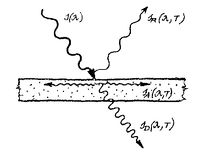
\includegraphics[width=5cm]{200px-Fenytores_homsug}
        \caption{Az elektromágneses sugárzás szétbomlása anyaggal való kölcsönhatás esetén \cite{leir}}
        \label{fig:0em}
    \end{figure}

    Ha a fogadó oldalt nézzük, egy testet érő elektromágneses sugárzással három dolog történhet: áteresztődik ($I_t(\lambda, T)$), elnyelődik ($I_a(\lambda, T)$), vagy visszaverődik ($I_r(\lambda, T)$), ahogy ezt~\aref{fig:0em}. ábrán is láthatjuk.
    Természetesen ez a három jelenség egyszerre lép fel a kölcsönhatások legnagyobb részében, így a végbemenetelüket valamilyen arányszámmal tudjuk jellemezni:
    \begin{align}
        &\xi(\lambda, T)=\frac{I_\xi(\lambda, T)}{I(\lambda)}; &\xi\in\{t, a, r\} \\
        &\xi(T)=\frac{\int_{0}^{\infty} I_\xi(\lambda, T)~\mathrm{d}\lambda}{\int_{0}^{\infty} I(\lambda)~\mathrm{d}\lambda}=\frac{I_\xi(T)}{I_0}.\label{eq:0intabs}
    \end{align}
    Ezeket rendre \textit{transzmisszió}-, \textit{abszorpció}- és \textit{reflexióképességnek} nevezzük.
    Mindet tudjuk definiálni integrált esetben is, ahogy \aref{eq:0intabs}. egyenletben látható.
    Az energiamegmaradásból következik, hogy a teljes intenzitás is megmarad, így:
    \begin{align}
        &t(\lambda, T)+a(\lambda, T)+r(\lambda, T)=1 \\
        &t(T)+a(T)+r(T)=1.
    \end{align}

    \subsection{Az abszolút fekete test}\label{subsec:az-abszolut-fekete-test}
    A testek sugárzásának vizsgálatához célszerű bevezetni egy absztrakciót (valójában ilyen test nem létezik), melyet \textbf{abszolút fekete testnek} hívunk.
    Ennek a legfontosabb tulajdonsága, hogy minden ráeső elektromágneses sugárzást elnyel, így felírható:
    \begin{equation}
        a(\lambda, T)=a(T)=1\equiv a_f.
    \end{equation}
    Fontos, hogy a fekete test által kisugárzott energia spektruma elméleti megfontolásokkal levezethető (\textit{Max Planck}, 1900 \cite{planck}):
    \begin{equation}
        \varepsilon_f(\lambda, T)=\frac{2hc^2}{\lambda^5}\frac{1}{e^{\frac{hc}{\lambda k_BT}}-1},
    \end{equation}
    ahol $h$ a Planck-állandó, $c$ a fénysebesség és $k_B$ a Boltzmann-állandó. Ez a \textbf{Planck-féle sugárzási törvény}.
    A megfelelő hullámhosszfüggés néhány hőmérsékleten \aref{fig:0blackrad}. ábrán látható. A maximumokra érvényes továbbá a \textbf{Wien-féle eltolódási törvény}, mely szerint:
    \begin{equation}
        \lambda_{\mathrm{max}}\cdot T=\mathrm{const}.
    \end{equation}
    \begin{figure}[H]
        \centering
        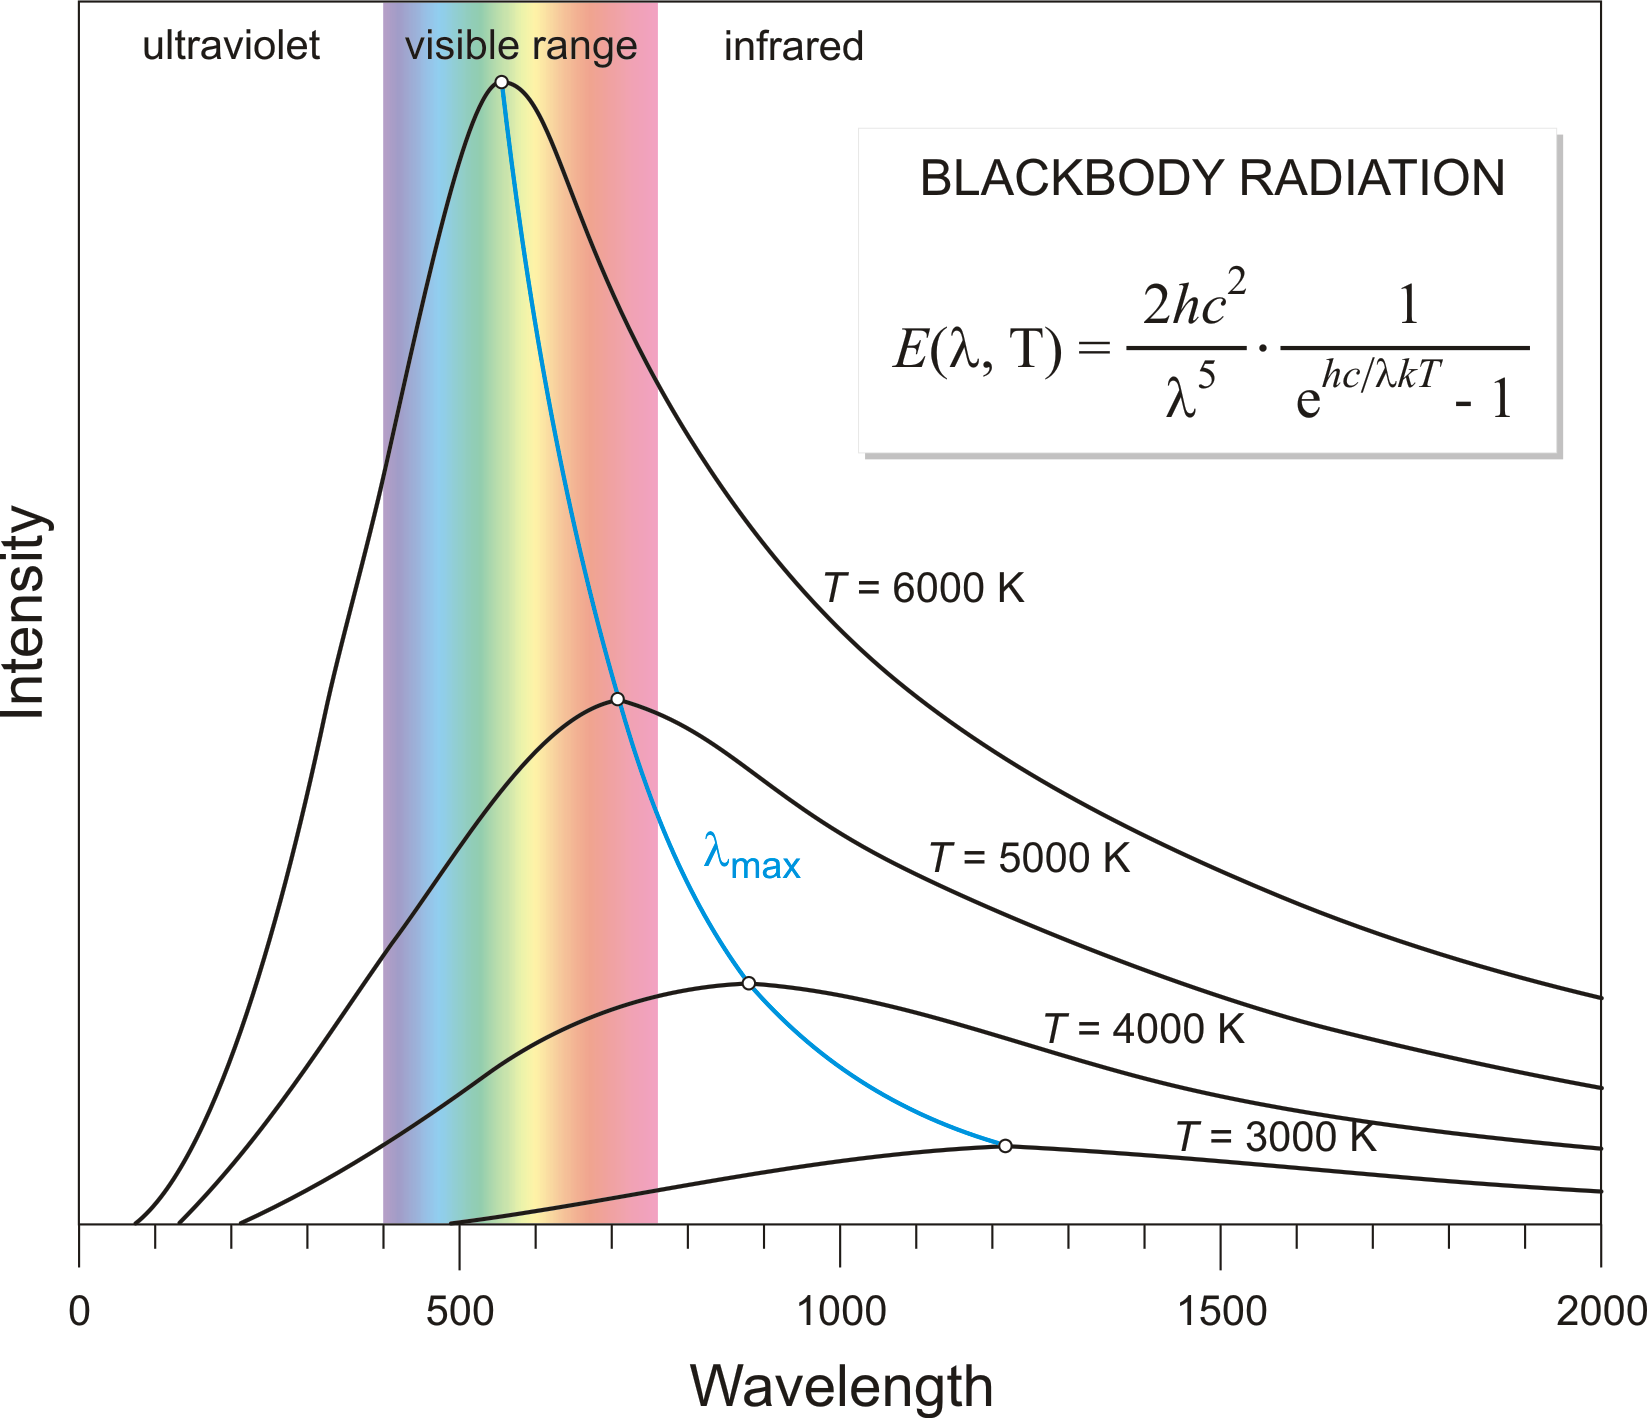
\includegraphics[width=8cm]{blackbody_radiation}
        \caption{A fekete test sugárzás szemléltetése különböző hőmérsékleteken \cite{rad}}
        \label{fig:0blackrad}
    \end{figure}

    A felületre normált sugárzási teljesítményt az $\varepsilon_f$ függvény hullámhossz szerinti integrálja adja meg, melyre érvényes a \textbf{Stefan-Boltzmann-törvény}:
    \begin{equation}
        E_f(T)=\int_{0}^{\infty} \varepsilon_f(\lambda, T)~\mathrm{d}\lambda=\sigma T^4.
    \end{equation}
    Eszerint a kisugárzott teljesítmény arányos a hőmérséklet negyedik hatványával, az arányosssági tényező pedig a \textit{Stefan-Boltzmann-állandó}: $\sigma=5.670\cdot10^{-8}~\frac{W}{m^2K^4}$.
    Egy felületről kisugárzott teljesítmény azonban nem minden irányba azonos, annak szögfüggését a \textit{Lambert-törvény} adja meg:
    \begin{equation}
        \mathrm{d}E_\varphi(T)=\sigma T^4\frac{\cos\varphi}{\pi}\mathrm{d}\Omega,
    \end{equation}
    ahol $\varphi$ a felület normálvektorával bezárt szög, $\mathrm{d}\Omega$ pedig a térszög, amelyet vizsgálunk.

    \subsection{Nem fekete testek sugárzása}
    Két tetszőleges ($1$, $2$) testre a tapasztalat szerint fennáll a következő összefüggés, a hőmérsékleti sugárzás \textit{Kirchhoff-törvénye}:
    \begin{equation}
        \frac{\varepsilon_1(\lambda, T)}{a_1(\lambda, T)}=\frac{\varepsilon_2(\lambda, T)}{a_2(\lambda, T)}=\mathrm{const}.
    \end{equation}
    Mivel ez a fekete testre is érvényes, bármely testre felírható:
    \begin{equation}
        \frac{\varepsilon(\lambda, T)}{a(\lambda, T)}=\varepsilon_f(\lambda, T),
    \end{equation}
    azaz az abszorpció- és emisszióképesség a másik ismeretében meghatározható.

    Szerencsére sok esetben még az egyiket sem kell meghatároznunk minden $\lambda$ értékre, mivel nem túl magas hőmérsékleten sok anyag esetében jó közelítéssel érvényes az $a(\lambda, T)\approx a(T)$ hullámhossz-függés elhanyagolás.
    Az ilyen testeket \textit{szürke testnek} hívjuk (természetesen ez nem a tényleges színre utal).
    Még tovább egyszerűsíthetjük a feladatot alacsony hőmérsékleten, mivel itt legtöbbször az abszorpciós tényező közel konstans, azaz $a(T)\approx a$.

    Ezen közelítések alkalmazásával már könnyen megkapható egy test integrált emisszióképessége:
    \begin{equation}
        E(T)=\int_{0}^{\infty} \varepsilon(\lambda, T)~\mathrm{d}\lambda=\int_{0}^{\infty} a(\lambda, T)\varepsilon_f(\lambda, T)~\mathrm{d}\lambda=a \int_{0}^{\infty} \varepsilon_f(\lambda, T)~\mathrm{d}\lambda,
    \end{equation}
    mely a \textit{Stefan-Boltzmann-törvény} alapján:
    \begin{equation}
        E(T)=a\sigma T^4.
    \end{equation}
    Alacsony hőmérsékletű szürke testekre igaz tehát, hogy integrált emisszióképességük csak egy konstans ($a\in[0, 1]$) szorzóban tér el a fekete testétől.

    \section{Előkészületek}
    A mérés elején megmértük a "Stefan-Boltzmann-izzó" és az alacsony hőmérsékletű sugárforrás ("kocka") érzékelő termisztorának kezdeti, hideg ellenállását.
    A termisztor ellenállása multiméterrel mérve $R_{t0}=84,45\pm 0,10~\mathrm{k\Omega}$-nak adódott, míg az izzó ellenállását annak kicsi volta miatt egy négypontos ellenállásmérővel mértük és $R_{s0}=0,274\pm 0,003~\Omega$ értéket kaptunk.

    Kiszámítottuk továbbá a leiratban (\cite{leir}) mellékelt táblázatok alapján az izzó ellenállásának és a kockában és az abszorpciómérőben lévő termisztorok ellenállásának hőmérsékletfüggését.
    Az izzó wolframszálának esetében a szobahőmérsékletre normált ellenállás ($\frac{R}{R_{300\mathrm{K}}}$) a vizsgált tartományban ($\approx300$-$3000$K) jó közelítéssel lineáris függést mutat, így ilyen alakú függvényt illesztettünk rá:
    \begin{equation}
        T\left(\frac{R}{R_{300\mathrm{K}}}\right)=(169,02\pm 1,54)\cdot\frac{R}{R_{300\mathrm{K}}}+(251,29\pm17,92)~\mathrm{K},
    \end{equation}
    ahol a paraméterek hibáit az illesztés kovarianciamátrixából határoztuk meg.

    A termisztor esetében már nem volt ilyen egyszerű dolgunk, mivel ennek tudottan nemlineáris az ellenállás-hőmérséklet karakterisztikája.
    Ettől függetlenül a kapott értékeket ábrázolva úgy gondoltuk, hogy a függés valamilyen hatványfüggvény szerinti lesz, a Python pedig sok ismeretlen paramétert is jól illeszt.
    Az így illesztett függvény a következő lett:
    \begin{equation}
        T(R_t)=\dfrac{745,55\pm 0,64}{R_t^{0,1350\pm 0,0003}}+(-132,66\pm 0,49)~\mathrm{K}.
    \end{equation}
    Az illesztések pontosságát \aref{fig:1ill}. ábra mutatja.
    Minden ezután következő feladatban ezen függésekből határoztuk meg a hőmérsékleteket a mért ellenállásértékekből.
    \begin{figure}[H]
        \centering
        \begin{subfigure}[b]{0.49\textwidth}
            \centering
            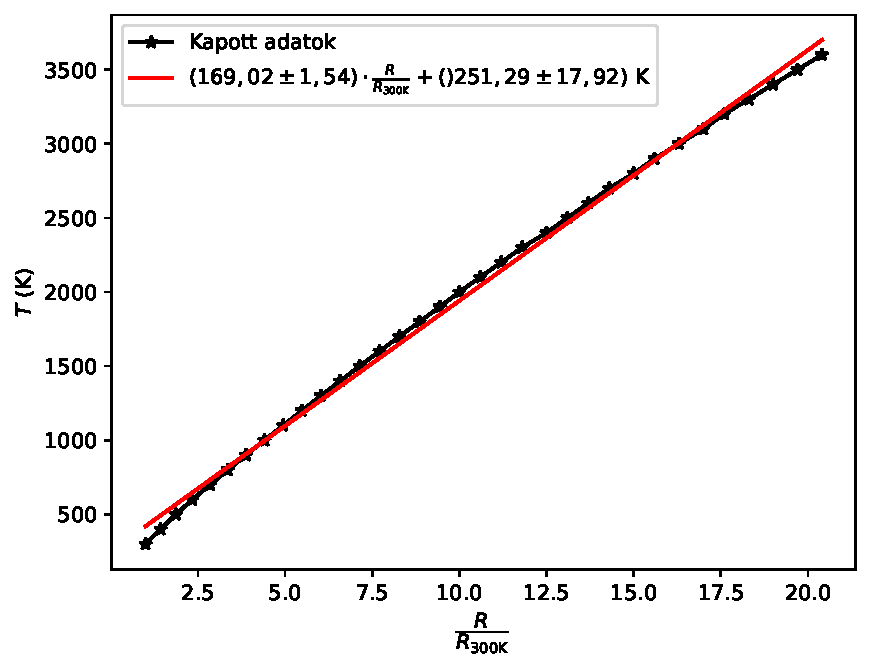
\includegraphics[width=\textwidth]{1linilleszt}
            \caption{A táblázatból kapott adatok és az illesztés az izzószál hőmérsékletének ellenállásfüggésére}
            \label{fig:1izzo}
        \end{subfigure}
        \begin{subfigure}[b]{0.49\textwidth}
            \centering
            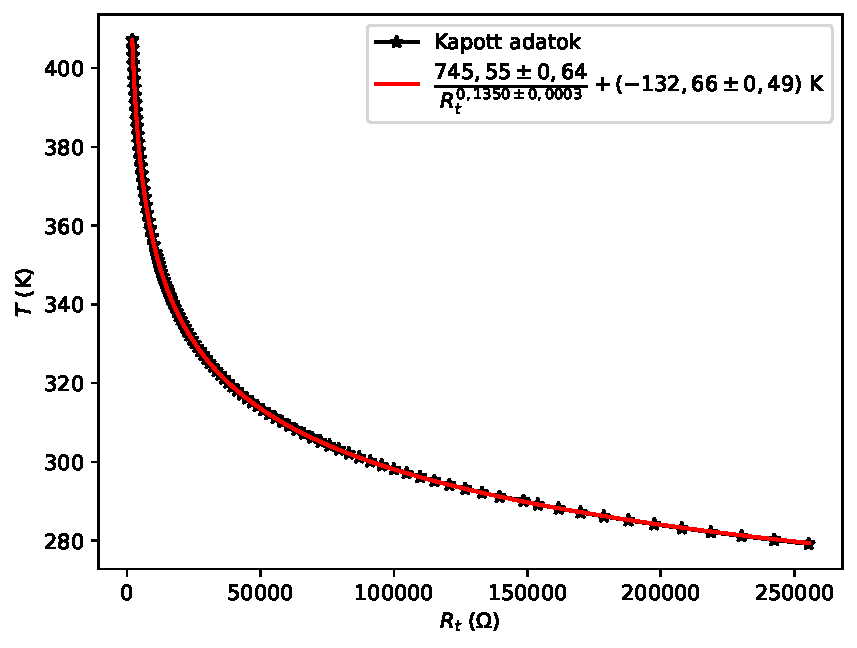
\includegraphics[width=\textwidth]{1vmiilleszt}
            \caption{A táblázatból kapott adatok és az illesztés a termisztor hőmérsékletének ellenállásfüggésére}
            \label{fig:1term}
        \end{subfigure}
        \caption{Az illesztett hőmérséklet-ellenállásfüggések}
        \label{fig:1ill}
    \end{figure}

    \section[Magas Hőmérsékletű Sugárforrás]{Stefan-Boltzmann-Törvény Ellenőrzése Magas Hőmérsékletű Sugárforrással}
    A méréshez szükség volt egy Stefan-Boltzmann izzóra, egy tápegységre, 3 db multiméterre, egy sugárzásdetektorra és az ehhez tartozó állványra, valamint vezetékekre.
    A mérési összeállítást \aref{fig:2fel}. ábra mutatja.
    \begin{figure}
        \label{fig:2fel}
        \centering
        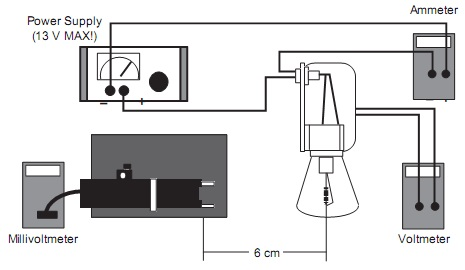
\includegraphics[width=6cm]{Mérési_elrendezés_1_homsug}
        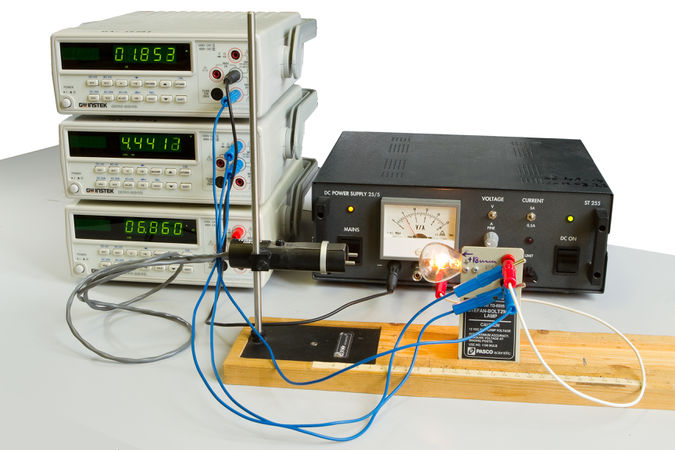
\includegraphics[width=6cm]{Homsug8.jpg}
        \caption{Bal oldalon a mérési összeállítás vázlata, jobb oldalon pedig a megvalósításról készült kép látható.}
    \end{figure}
    \par
    Ahogy az a képen is látható, mértük az izzó $I_{\mathrm{izzó}}$ áramát (20~A-es méréshatár), a rajta eső $U_{\mathrm{izzó}}$
    feszültséget, valamint a detektor $U'_{\mathrm{det}}$ feszültségét (200~mV-os méréshatár). A detektort mindig árnyékoltuk, amikor éppen nem végeztünk mérést,
    ezzel elkerülve az érzékelő felmelegedését. A mért detektorfeszültségből automatikusan levontuk a detektor sötétáramához tartozó feszültséget ($U_{\mathrm{sötét}}=0,13$~mV),
    így a sugárzással arányos kimenőjelet kaptunk ($U_{\mathrm{det}}$).
    Az izzóra kapcsolt feszültséget 1 V-os lépésekben 1 V-ról 12 V-ra növeltük, közben a mért áram- és feszültségértékekből kiszámoltuk az izzó ellenállását,
    majd a táblázat alapján meghatároztuk a hőméréskletét. Ehhez a megadott adatokra (Fizipédia, A volfram fajlagos ellenállásának a hőmérsékletfüggése táblázat \cite{leir})
    megfelelő alakú függvényt illesztettünk.
    Mért adatainkat \aref{tab:2fel}. táblázat tartalmazza.

    \begin{tabular}{cccccc}
        \toprule
        $I_{\mathrm{izzó}}$ (A) & $U_{\mathrm{izzó}}$ (V) & $R_{\mathrm{izzó}}$ (Ohm) & $U_{\mathrm{det}}$ (mV) & $R_{\mathrm{izzó}}/R_0$ & T (K) \\
        \midrule
        0,980000 & 1,000000 & 1,020000 & 0,070000 & 3,710000 & 878,800000 \\
        1,310000 & 2,000000 & 1,530000 & 0,920000 & 5,590000 & 1195,670000 \\
        1,570000 & 3,000000 & 1,910000 & 2,580000 & 6,990000 & 1431,980000 \\
        1,830000 & 4,030000 & 2,200000 & 5,370000 & 8,040000 & 1610,550000 \\
        2,040000 & 5,000000 & 2,450000 & 8,090000 & 8,940000 & 1763,050000 \\
        2,240000 & 6,030000 & 2,690000 & 11,480000 & 9,810000 & 1909,730000 \\
        2,420000 & 6,980000 & 2,890000 & 14,970000 & 10,530000 & 2031,020000 \\
        2,600000 & 8,040000 & 3,090000 & 19,320000 & 11,290000 & 2158,820000 \\
        2,760000 & 9,000000 & 3,260000 & 23,270000 & 11,900000 & 2263,030000 \\
        2,920000 & 10,010000 & 3,430000 & 27,830000 & 12,510000 & 2365,230000 \\
        3,070000 & 11,000000 & 3,580000 & 32,760000 & 13,080000 & 2462,160000 \\
        3,210000 & 11,970000 & 3,730000 & 37,510000 & 13,610000 & 2551,420000 \\
        \bottomrule
        \label{tab:2fel}
    \end{tabular}
    \par
    A detektorfeszültséget ábrázolva a kiszámított hőmérséklet negyedik hatványának függvényében egy egyenest kapunk (ld. \aref{fig:2fel2}. ábra),
    melynek egyenlete $(9,11 \cdot 10^{-16} \pm 5,45 \cdot 10^{-18})[V/K^4] \cdot T^4 -(7,368 \cdot 10^{-4} pm 1,21 \cdot 10^{-4})[V].
    A paraméterek hibáját az illesztés kovarianciamátrixából határoztuk meg.
    Megállapítható, hogy mivel a detektorfeszültség (mely arányos a kisugárzott energiával) arányos a hőmérséklet negyedik hatványával,
    így a Stefan-Boltzmann törvény teljesül.
    \begin{figure}
        \label{fig:2fel2}
        \centering
        \includegraphics[width=6cm]{2fel.pdf}
        \caption{A detektorfeszültség függése $T^4$-től.}
    \end{figure}




    \section[Intenzitás Távolságfüggése]{Pontszerű Forrás Sugárzási Intenzitásának Távolságfüggése}

    
    \section[Alacsony Hőmérsékletű Sugárforrás]{Stefan-Boltzmann-Törvény Ellenőrzése Alacsony Hőmérsékletű Sugárforrással}
    Ebben a feladatban egy alacsony hőmérsékletű sugárforrás (továbbiakban: \textit{kocka}) emissziójának vizsgálatával ellenőriztük a \textit{Stefan-Boltzmann-törvény} fennállását és határoztuk meg a kocka relatív emissziós (abszorpciós) tényezőjét.

    \subsection{A mérési összeállítás}
    \begin{figure}[H]
        \centering
        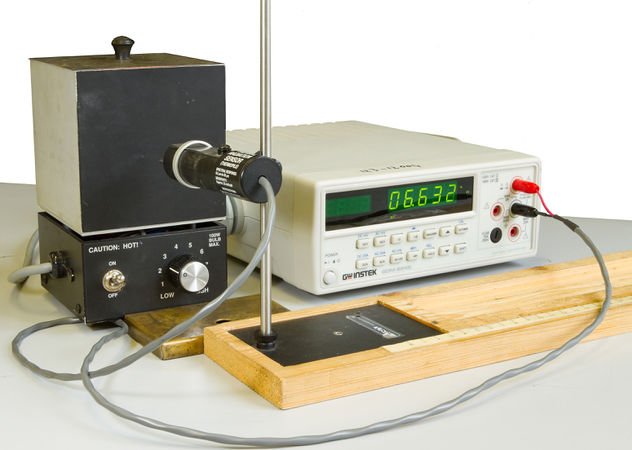
\includegraphics[width=8cm]{632px-Homsug5}
        \caption{Mérési összeállítás a kocka emissziójának vizsgálatához}
        \label{fig:4ossze}
    \end{figure}

    A méréshez \aref{fig:4ossze}. ábrán látható módon szembe állítottuk a detektort a kockával, attól nagyjából 4 cm távolságban.
    A detektor feszültségét ($U_d$) egy multiméteren néztük, a kocka termisztorának ellenállását ($R_t$) pedig egy másikon.
    Kezdetben (ekkor még nem kapcsoltuk be a kocka fűtését) a kocka ellenállása $R_{t0}=80,13\pm 0,10~\mathrm{k\Omega}$ volt.
    Ezután \textit{HIGH} állásba kapcsoltuk a kocka fűtését, és megkezdtük a mérést.

    \subsection{A mérés menete}
    A mérés során fél percenként forgattuk a kockát, melynek felületei így a következő sorban kerültek sorra: feketére festett, matt alumínium, fehérre festett, majd polírozott alumínium.
    Minden pozícióban feljegyeztük a detektor $U_d$ feszültségét és a kocka termisztorának pillanatnyi $R_t$ ellenállását.
    A mérést addig végeztük, amíg a termisztor ellenállása már nem igazán változott és a kezünknek is elég volt a forró kocka forgatásából (a kocka alja is jól felmelegedett).


    \section{Abszorpciós tényezők meghatározása}

    \begin{thebibliography}

        \bibitem{leir} \href{https://fizipedia.bme.hu/index.php/H%C5%91m%C3%A9rs%C3%A9kleti_sug%C3%A1rz%C3%A1s_vizsg%C3%A1lata}{Fizipédia, mérési leirat}
        \bibitem{planck} \href{https://en.wikipedia.org/wiki/Planck%27s_law}{A Planck-féle sugárzási törvény}
        \bibitem{rad} \href{https://glossary.periodni.com/glossary.php?en=blackbody+radiation}{A fekete test sugárzása}
    \end{thebibliography}

\end{document}